\documentclass[11pt]{article}
\usepackage{icmlko}
\begin{document}

\title{달력은 집에서만 일한다 --- 그리고 내가 쓴 합격 기준을 물린다}
\author{월드모델 실험실}
\date{노트 439 · 2026년 8월 6일}
\maketitle

\begin{abstract}
노트 438의 곁가지 --- KR 만화에 달력 축 여섯을 붙이자 전이가 두 팔 다
$-0.05$ 내렸다 --- 를 LODO 열한 짝으로 제대로 물었다. 이 실험실에 오래
열려 있던 갈래(``달력이 왜 트리에서만 되는지, 설명 넷 실패'')와 같은 자리다.

\begin{center}
\begin{tabular}{lr}
\hline
달력을 빼서 전이가 오른 도메인 & $5/11$ \\
평균 & $\mathbf{+0.0005}$ \\
잡음 문턱($0.0108$)을 넘는 것 & $4$ 개 (양수 3 · 음수 1) \\
\hline
\end{tabular}
\end{center}

\textbf{대본은 ``통과''라 찍었다. 안 받는다.} 사전 등록에 ``문턱 넘는 것 중
다수가 양수''라고 \emph{느슨하게} 적어 둔 탓이다 --- 넷 중 셋이 양수일 우연
확률이 $\mathbf{0.312}$ 다. \textbf{$n{=}4$ 짜리 다수결은 다수결이 아니다.}

정직한 판정은 \textbf{중립}이다. KR 만화의 $-0.05$ 는 그 도메인 하나의 일이고
달력은 안 본 도메인에 해롭지 않다.
\end{abstract}

\section{그런데 이롭지도 않다}

중립이라는 것 자체가 이 갈래에 답을 하나 준다.

\begin{center}
\begin{tabular}{lr}
\hline
달력 축이 \textbf{판}에 주는 값 & $+0.0205$ (노트 213) \\
달력 축이 \textbf{전이}에 주는 값 & $+0.0005$ (여기, 열한 짝 평균) \\
\hline
\textbf{비} & $\mathbf{41}$ 배 \\
\hline
\end{tabular}
\end{center}

\textbf{달력은 학습 도메인 안에서 일하고 안 본 도메인에는 아무것도 주지
않는다.} 열린 갈래의 이름(``트리에서만 되는'')이 가리키던 것과 방향이 맞는다
--- 다만 여기서 잰 것은 모형 종류가 아니라 \textbf{도메인 안팎}이다.

노트 213이 달력의 값을 지켰을 때 근거는 판이었다. 그 값은 그대로다.
\textbf{챔피언에서 뺄 이유가 없다} --- 전이를 해치지 않으므로.

\section{내가 쓴 기준의 흠}

노트 434가 ``$|\Delta| > 3\times$ 짝 잡음인 도메인만 센다''는 문턱을 달았다.
좋았다. 그런데 이번 사전 등록에서 \textbf{문턱을 넘는 도메인이 몇이든 그 중
다수면 통과}라고 썼다. 넷만 넘으면 셋으로 통과다.

\begin{center}
\textbf{문턱을 통과한 도메인 수가 적으면 다수결 자체가 성립하지 않는다.}\\
셀 도메인이 $\ge 6$ 개일 때만 다수결을 적는다. 그 아래는 ``잴 수 없음''이다.
\end{center}

노트 378 ④(``채점 집합이 다르면 미결정이 아니라 잴 수 없음'')와 같은 정신이다.
\textbf{미결정과 잴 수 없음은 다르다.}

\begin{tabular}{lp{7.0cm}}
\hline
달력 & \textbf{판에서만 값이 있다.} 챔피언 유지. 열린 갈래에 한 줄 보탠다 \\
문턱 넘는 도메인이 적은 것 & 이번엔 넷이었다. \textbf{씨앗을 늘리면 문턱이
내려가 더 많이 센다} --- 노트 434가 적어 둔 그 일이 이제 두 번째로 걸린다 \\
집 밖 둘 & 넷째 설명까지 죽었고(노트 438) 언어만 다른 도메인이 없다 \\
\hline
\end{tabular}

\begin{figure}[h]
\centering
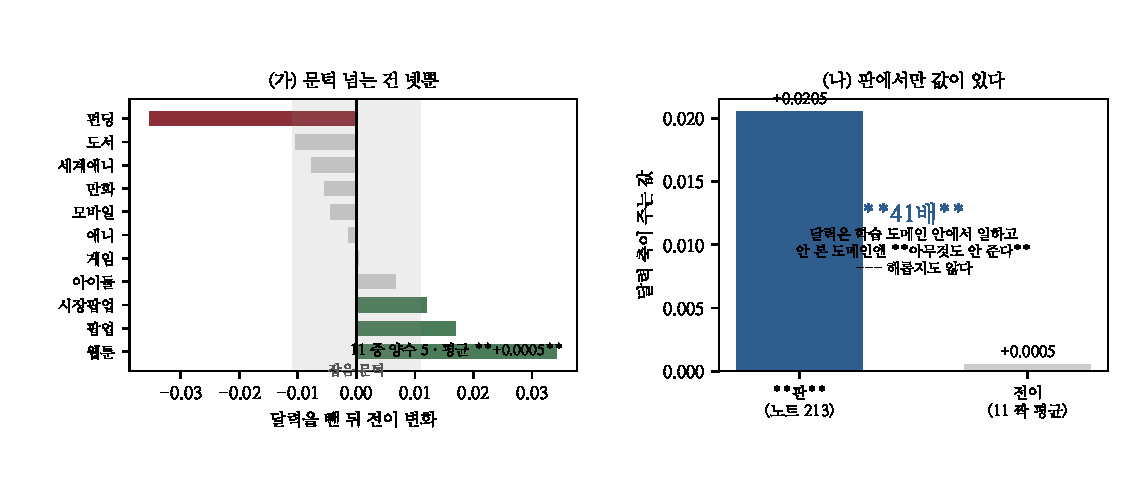
\includegraphics[width=\textwidth]{figs/fig439.pdf}
\caption{(가) 잡음 문턱(회색 띠)을 넘는 도메인은 넷뿐. (나) 달력은 판에
$+0.0205$, 전이에 $+0.0005$ --- 41배.}
\end{figure}

\end{document}
